\documentclass[9pt]{beamer}

\usepackage[T1]{fontenc}
\usepackage[utf8]{inputenc}
\usepackage[frenchb]{babel}
\usepackage{eurosym}

\usepackage{multirow}

\usepackage{graphicx}


\newcommand\host{{\it host} }
\newcommand\device{{\it device} }


% --------- BEGIN STYLE BEAMER ---------
\usetheme{Madrid}
\definecolor{ECNBleu}{HTML}{102648}
\definecolor{ECNJaune}{HTML}{FAB600}

\setbeamercolor{frametitle}{bg=ECNBleu,fg=white} %le titre de la frame, en haut
\setbeamercolor{title in head/foot}{bg=ECNJaune,fg=ECNBleu} %barre bas, milieu
\setbeamercolor{author in head/foot}{bg=ECNBleu,fg=ECNJaune} %barre bas, gauche
\setbeamercolor{date in head/foot}{bg=ECNBleu,fg=ECNJaune} %barre bas, droit
\setbeamercolor{section in head/foot}{bg=ECNJaune,fg=ECNBleu} %haut gauche
\setbeamercolor{subsection in head/foot}{bg=ECNBleu,fg=ECNBleu} %haut droite
\setbeamercolor{title}{bg=ECNBleu,fg=white}
\setbeamercolor{block title}{fg=white,bg=ECNBleu}

%\setbeamercolor{normal text}{bg=IUTBleuFonce} %texte
\setbeamercolor{item}{bg=ECNBleu}
\setbeamercolor{subitem}{bg=ECNJaune}
\setbeamercolor{description item}{fg=couleurEmph}
\setbeamercolor{section in toc}{fg=ECNBleu}
%\setbeamercolor{subsubitem}{bg=IUTBleuFonce}

%structure (eq emph dans beamer)
\setbeamercolor{emph}{fg=couleurEmph}
% ----------------------------

\usepackage{listings}

\lstdefinestyle{customc}{
  belowcaptionskip=1\baselineskip,
  breaklines=true,
  frame=L,
  xleftmargin=\parindent,
  language=C,
  showstringspaces=false,
  basicstyle=\tiny\ttfamily,
  keywordstyle=\bfseries\color{green!40!black},
  commentstyle=\itshape\color{purple!40!black},
  identifierstyle=\color{blue},
  stringstyle=\color{orange},
}

\lstset{escapechar=@,style=customc}

\newenvironment<>{questionblock}[1]{%
\setbeamercolor{block title}{bg=ECNJaune,fg=ECNBleu}%
\begin{block}#2{#1}}{\end{block}}

\title[GPGPU]{Programmation sur Processeur Graphique}

\subtitle[\ldots]{
---\\Partie 7 : Le retour de la gestion de la mémoire\\(Pinned et Unified Memory)}
\author[P.-E. Hladik]{Pierre-Emmanuel Hladik\\\tiny pierre-emmanuel.hladik@ec-nantes.fr}
\institute[Centrale Nantes]{}
\date{\today}

\begin{document}

 \frame{\titlepage}
 

\begin{frame}[plain]
\frametitle{Retour sur les transferts mémoire CPU-GPU}

\begin{block}{}
Pour être efficace, l'appel à {\tt cudaMemcpy()} utilise une unité matérielle {\bf DMA (Direct Memory Access)}.
\end{block}

\begin{block}{DMA}
L'accès direct à la mémoire DMA (Direct Memory Access) est un procédé informatique où des données circulant de, ou vers, un périphérique (port de communication, disque dur, etc.) sont transférées directement par un contrôleur adapté vers la mémoire principale de la machine, sans intervention du microprocesseur si ce n'est pour lancer et conclure le transfert. [\href{https://fr.wikipedia.org/wiki/Accès_direct_à_la_mémoire}{wikipedia}]
\end{block}

Le DMA utilise les adresses physiques :
	\begin{itemize}
		\item L'adresse est traduite et la présence de la page est vérifiée pour l'ensemble des régions source et destination au début de chaque transfert DMA.
		\item Aucune traduction d'adresse pour le reste du même transfert DMA, ce qui permet d'obtenir une grande efficacité.
	\end{itemize}
	


\end{frame}

 %%%%%%%%%%%%%%%%%%%%%%%%%%
\begin{frame}[plain]
\frametitle{Utilisation d'une mémoire épinglée (pinned)}

	\begin{alertblock}{}
	Le système d'exploitation peut accidentellement supprimer les données lues ou écrites par un DMA et insérer une autre {\bf page virtuelle}\footnote{ou comment gérer un espace mémoire plus grand que la mémoire vive...} au même emplacement physique.
	\end{alertblock}
	
		\begin{block}{Mémoire épinglée (pinned) [idem Page Locked Memory, Locked Pages, etc.]}
		 La mémoire épinglée est constituée de pages de mémoire virtuelle qui sont marquées ---appel système {\tt mlockall()}--- de manière à ne pas pouvoir être retirées par pagination
	\end{block}


	\begin{block}{}
	 	Le DMA utilisé par {\tt cudaMemcpy()} nécessite que toute source ou destination dans la mémoire de l'hôte soit allouée en tant que mémoire épinglée : 		
			\begin{itemize}
		\item  Lors d'un appel à {\tt cudaMemcpy()}, si une source ou une destination dans la mémoire de l'hôte n'est pas allouée en mémoire épinglée, elle doit d'abord être copiée dans une mémoire épinglée (surcharge supplémentaire)
		\item {\tt cudaMemcpy()} est plus rapide si la source ou la destination de la mémoire hôte est allouée en mémoire épinglée, car aucune copie supplémentaire n'est nécessaire.
	\end{itemize}
	\end{block}

	

\end{frame}

 %%%%%%%%%%%%%%%%%%%%%%%%%%
\begin{frame}[plain]
\frametitle{Utilisation de la mémoire épinglée dans CUDA}

\begin{block}{Fonction CUDA pour déclarer un espace de mémoire épinglée}
\begin{itemize}
\item  La fonction {\tt cudaHostAlloc ( void** pHost, size\_t size, unsigned int  flags )} alloue un espace de {\bf mémoire épinglée pour l'host}, avec :
	\begin{itemize}
		\item {\tt pHost} : Adresse du pointeur vers la mémoire allouée
		\item {\tt size} : Taille de la mémoire allouée en octets
		\item {\tt flags} : Option à utiliser {\tt cudaHostAllocDefault}
	\end{itemize}
\item La fonction {\tt cudaFreeHost(void* ptr)} libre un espace de mémoire épinglée avec {\tt ptr} le pointeur vers la mémoire à libérer.
\end{itemize}
\end{block}

	\begin{itemize}
		\item La mémoire allouée est utilisée sur l'\host de la même manière que celle créée avec {\tt malloc()} et {\tt free()}
		\item  La seule différence est que la mémoire allouée ne peut pas être paginée par le système d'exploitation
		\item  La fonction {\tt cudaMemcpy()} est environ 2 fois plus rapide avec de la mémoire épinglée
	\end{itemize}

\begin{alertblock}{}
La mémoire épinglée est une ressource limitée. Une sur-utilisation peut avoir de graves conséquences. \`A consommer avec modération.
\end{alertblock}

\end{frame}
%%%%%%%%%%%%%%%%%%%%%%%%%%
\begin{frame}[plain,fragile]
\frametitle{Exemple de programme sans mémoire épinglée}


\lstset{escapechar=@} 
\begin{lstlisting}[language=C]
__global__ void AplusB(int *ret, int a, int b) {
    ret[threadIdx.x] = a + b + threadIdx.x;
}

int main() {
    int *h_ret = (int *)malloc(1000 * sizeof(int));    
    
    // Creation de l'espace memoire sur le GPU
    int *d_ret;
    cudaMalloc(&d_ret, 1000 * sizeof(int));
    
    AplusB<<< 1, 1000 >>>(d_ret, 10, 100);

    // Transfert explicite de la memoire du GPU vers le CPU
    cudaMemcpy(h_ret, d_ret, 1000 * sizeof(int), cudaMemcpyDefault);
    
    for(int i = 0; i < 1000; i++) {
        printf("%d: A+B = %d\n", i, host_ret[i]); 
    }
      
    free(host_ret);
    cudaFree(ret); 
    return 0;
}
 \end{lstlisting}

\end{frame}
%%%%%%%%%%%%%%%%%%%%%%%%%%
\begin{frame}[plain,fragile]
\frametitle{Exemple de programme avec mémoire épinglée}


\begin{lstlisting}[language=C]
__global__ void AplusB(int *ret, int a, int b) {
    ret[threadIdx.x] = a + b + threadIdx.x;
}

int main() {

    // Reservation d'un espace epingle sur le CPU    
    int *h_ret;
    cudaHostAlloc((void **) &h_ret, 1000 * sizeof(int), cudaHostAllocDefault);    
    
    // Creation de l'espace memoire sur le GPU
    int *d_ret;
    cudaMalloc(&d_ret, 1000 * sizeof(int));
    
    AplusB<<< 1, 1000 >>>(d_ret, 10, 100);

    // Transfert explicite de la memoire du GPU vers le CPU
    cudaMemcpy(h_ret, d_ret, 1000 * sizeof(int), cudaMemcpyDefault);
    
    for(int i = 0; i < 1000; i++) {
        printf("%d: A+B = %d\n", i, host_ret[i]); 
    }
      
    cudaFreeHost(host_ret);     // Liberation de la memoire epinglee
    cudaFree(ret); 
    return 0;
}
 \end{lstlisting}

\end{frame}
%%%%%%%%%%%%%%%%%%%%%%%%%%


%%%%%%%%%%%%%%%%%%%%%%%%%%
\begin{frame}[plain]
\frametitle{Unified Memory}

\begin{itemize}
	\item La mémoire unifiée a été introduite pour la première fois dans CUDA 6.0\vspace{0.5em}

	\item C'est un espace mémoire commun qui est vu par l'\host et les {\it devices} comme une mémoire unique avec un espace d'adressage commun\vspace{0.5em}

	\item Le matériel/logiciel gère la migration des données automatiquement entre l'\host et le \device en maintenant la cohérence entre eux sans effectuer des appels explicites de copie de mémoire (i.e. élimine l'appel à la routine {\tt cudaMemcpy})\vspace{0.5em}

	\item La mémoire unifiée permet de :
	\begin{itemize}
		\item simplifier la programmation GPU en unifiant les espaces mémoire de manière cohérente
		\item maximiser la vitesse d'accès aux données par la migration transparente des données vers le processeur qui les utilise
	\end{itemize}
\end{itemize}
\end{frame}
%%%%%%%%%%%%%%%%%%%%%%%%%%
\begin{frame}[plain,fragile]
\frametitle{Exigence système}

La mémoire unifiée est disponible pour :
\begin{itemize}
	\item un GPU avec une architecture 3.0 ou supérieure (classe Kepler ou plus récente)
	\item une application hôte 64 bits et un système d'exploitation adéquat (Linux ou Windows).
\end{itemize}

\end{frame}
%%%%%%%%%%%%%%%%%%%%%%%%%%
\begin{frame}[plain,fragile]
\frametitle{Routines d'utilisation}


\begin{itemize}
	\item Il n'est plus nécessaire de procéder à des transferts de mémoire explicites entre l'hôte et le périphérique. Toute allocation créée dans l'espace mémoire est automatiquement migrée vers l'endroit où elle est nécessaire.\vspace{0.5em}
	
	\item Un programme alloue la mémoire de deux manières : 
	\begin{itemize}
		\item via la routine {\tt cudaMallocManaged()}, qui est sémantiquement similaire à {\tt cudaMalloc()} ; ou 
		\item en définissant une variable globale {\tt \_\_managed\_\_}, qui est sémantiquement similaire à une variable {\_\_device\_\_}
	\end{itemize}
\end{itemize}

\end{frame}
%%%%%%%%%%%%%%%%%%%%%%%%%%

%%%%%%%%%%%%%%%%%%%%%%%%%%
\begin{frame}[plain,fragile]
\frametitle{Exemple de programme sans mémoire unifiée}


\lstset{escapechar=@} 
\begin{lstlisting}[language=C]
__global__ void AplusB(int *ret, int a, int b) {
    ret[threadIdx.x] = a + b + threadIdx.x;
}

int main() {
    int *h_ret = (int *)malloc(1000 * sizeof(int));    
    
    // Creation de l'espace memoire sur le GPU
    int *d_ret;
    cudaMalloc(&d_ret, 1000 * sizeof(int));
    
    AplusB<<< 1, 1000 >>>(d_ret, 10, 100);

    // Transfert explicite de la memoire du GPU vers le CPU
    cudaMemcpy(h_ret, d_ret, 1000 * sizeof(int), cudaMemcpyDefault);
    
    for(int i = 0; i < 1000; i++)
        printf("%d: A+B = %d\n", i, host_ret[i]); 
    free(host_ret);
    cudaFree(ret); 
    return 0;
}
 \end{lstlisting}

\end{frame}
%%%%%%%%%%%%%%%%%%%%%%%%%%
\begin{frame}[plain,fragile]
\frametitle{Exemple d'utilisation de {\tt cudaMallocManaged}}


\lstset{escapechar=@} 
\begin{lstlisting}[language=C]
__global__ void AplusB(int *ret, int a, int b) {
    ret[threadIdx.x] = a + b + threadIdx.x;
}

int main() {
    int *ret; // adresse commune CPU ET GPU
    
    @\textcolor{red}{cudaMallocManaged(\&ret, 1000 * sizeof(int))}@;
    
    AplusB<<< 1, 1000 >>>(ret, 10, 100);

    @\textcolor{red}{cudaDeviceSynchronize()}@;
    
    for(int i = 0; i < 1000; i++)
        printf("%d: A+B = %d\n", i, ret[i]);
    cudaFree(ret); 
    return 0;
}
 \end{lstlisting}
 
 \begin{itemize}
	\item La routine {\tt cudaMallocManaged()} renvoie un pointeur valable à la fois pour le code de \host et celui du \device. Cela permet d'utiliser {\tt ret} sans une copie séparée de {\tt host\_ret} ce qui simplifie et réduit la taille du programme\vspace{0.5em}

	\item Dans l'exemple non unifié, la routine {\tt cudaMemcpy()} est utilisée à la fois pour synchroniser le kernel (c'est-à-dire pour attendre qu'il finisse de fonctionner), et pour transférer les données vers l'hôte. L'utilisation de la mémoire unifiée nécessite donc un {\tt cudaDeviceSynchronize()}explicite avant que le programme hôte puisse utiliser en toute sécurité la sortie du GPU
 \end{itemize}

\end{frame}
%%%%%%%%%%%%%%%%%%%%%%%%%%
\begin{frame}[plain,fragile]
\frametitle{Exemple d'utilisation de {\tt \_\_managed\_\_}}


\lstset{escapechar=@} 
\begin{lstlisting}[language=C]
__device__ __managed__ int ret[1000]; // adresse globale commune CPU ET GPU

__global__ void AplusB(int a, int b) {
    ret[threadIdx.x] = a + b + threadIdx.x;
}

int main() {
    AplusB<<< 1, 1000 >>>(10, 100);

    @\textcolor{red}{cudaDeviceSynchronize()}@;
    
    for(int i = 0; i < 1000; i++)
        printf("%d: A+B = %d\n", i, ret[i]);
    return 0;
}
 \end{lstlisting}
 
Simplifie davantage un programme lorsque des variables globales sont utilisées.\vspace{0.5em}

Absence de l'appel à {\tt cudaMemcpy()} et le tableau de retour {\tt ret} est visible à la fois sur le CPU et le GPU.

\end{frame}
%%%%%%%%%%%%%%%%%%%%%%%%%%


%%%%%%%%%%%%%%%%%%%%%%%%%%
\begin{frame}[plain,fragile]
\frametitle{Migration et cohérence des données}

\begin{itemize}
	\item La mémoire unifiée tente d'optimiser les performances de la mémoire en déplaçant les données vers la mémoire \host si le CPU y accède et vers la mémoire du \device si le GPU y accède\vspace{0.5em}
	
	\item La migration des données est transparente pour un programme. Le système essaie de placer les données à l'endroit où elles sont le plus efficacement accessibles sans violer la cohérence\vspace{0.5em}
	
	\item L'emplacement physique des données est invisible pour un programme et peut être modifié à tout moment, mais les accès à l'adresse virtuelle des données resteront valides et cohérents à partir de n'importe quel processeur, indépendamment de la localité. {\bf La cohérence est l'exigence principale, avant les performances}\vspace{0.5em}
	
	\item Les architectures de GPU dont la capacité de calcul est inférieure à 6.x ne prennent pas en charge le déplacement fin des données gérées vers le GPU à la demande. Chaque fois qu'un kernel GPU est lancé, toute la mémoire gérée doit généralement être transférée vers la mémoire du GPU pour éviter les erreurs d'accès à la mémoire
\end{itemize}

\end{frame}
%%%%%%%%%%%%%%%%%%%%%%%%%%
\begin{frame}[plain]
\frametitle{Un peu de pratique avec le TD 7}

\begin{block}{Objectifs}
\begin{itemize}
	\item Déclaration d'un espace épinglé
	\item Utilisation de la mémoire unifiée
	\item Comparaison des performances
\end{itemize}
\end{block}
\end{frame}
%%%%%%%%%%%%%%%%%%%%%%%%%%

%%%%%%%%%%%%%%%%%%%%%%%%%%
\begin{frame}[plain]
\frametitle{Ouverture (très rapide) à la gestion de la mémoire}

\center Pour ceux qui souhaitent aller plus loin...

\end{frame}


  %%%%%%%%%%%%%%%%%%%%%%%%%%
\begin{frame}[plain]
\frametitle{Hiérarchie mémoire}

\begin{block}{}
	\begin{itemize}
		\item mégaoctet de mémoire cache volatile : rapide et chère
		\item gigaoctet de mémoire volatile de rapidité d'accès et prix moyen
		\item teraoctet de mémoire de masse non volatile lente et peu chère
	\end{itemize}
\end{block}

\begin{block}{Gestionnaire de mémoire}
Un gestionnaire de mémoire est l'entité d'un système d'exploitation qui gère la hiérarchie mémoire et la coordination entre elles.
\end{block}

\end{frame}

 
 %%%%%%%%%%%%%%%%%%%%%%%%%%
\begin{frame}[plain]
\frametitle{Structure de la mémoire associée à un programme}

\begin{center}
	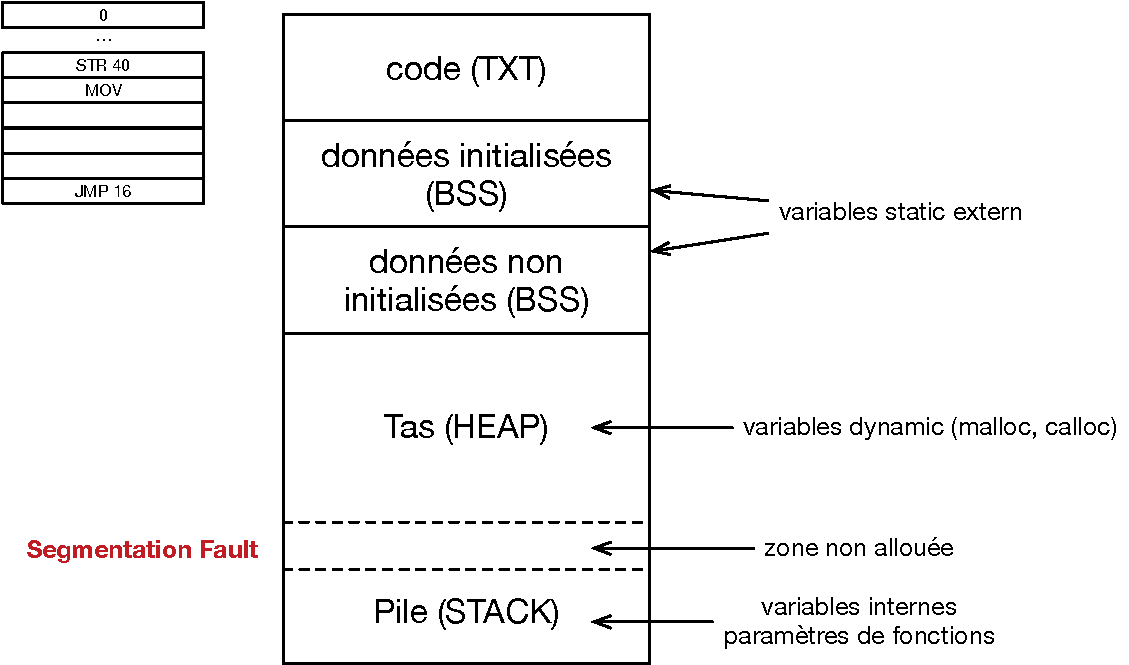
\includegraphics[scale=0.6]{./figures-pdf/section_memoire}
\end{center}

\end{frame}

 %%%%%%%%%%%%%%%%%%%%%%%%%%
\begin{frame}[plain,fragile]
\frametitle{Exemple : Structure de la mémoire associée à un programme}

\begin{columns}[t]
  \begin{column}{0.45\textwidth}
   	\begin{center}
		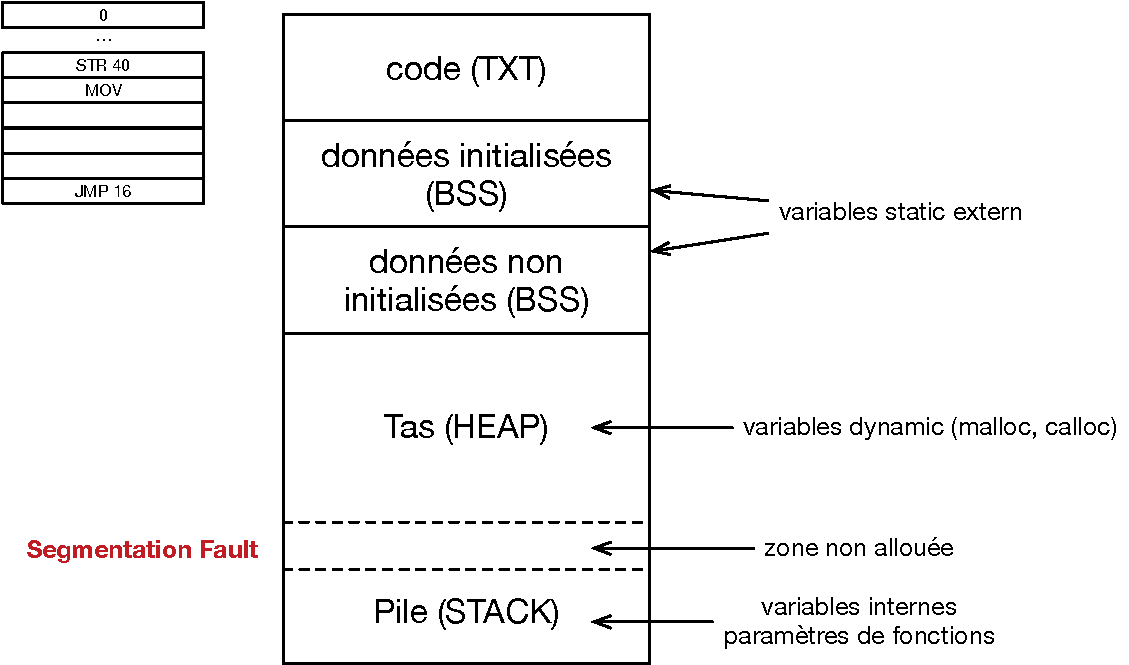
\includegraphics[scale=0.3]{./figures-pdf/section_memoire}
	\end{center}
  \end{column}
  
  \begin{column}{0.45\textwidth}
\begin{lstlisting}[language=C]
const int a  = 42;
int b[] = { 1, 2, 3 };
int c;

int f(int x, int y)
{
    int *z;
    malloc(z, sizeof(int));
    *z = x;
    *z = *z * y;
    return *z;
}

int main(int argc, char **argv)
{
    const int d = 1664;

    c = f(a, d);
    
    return 0;
}
 \end{lstlisting}

  \end{column}
 \end{columns}  

\end{frame}

 %%%%%%%%%%%%%%%%%%%%%%%%%%
\begin{frame}[plain]
\frametitle{Et avec plusieurs programmes...}

\begin{center}
	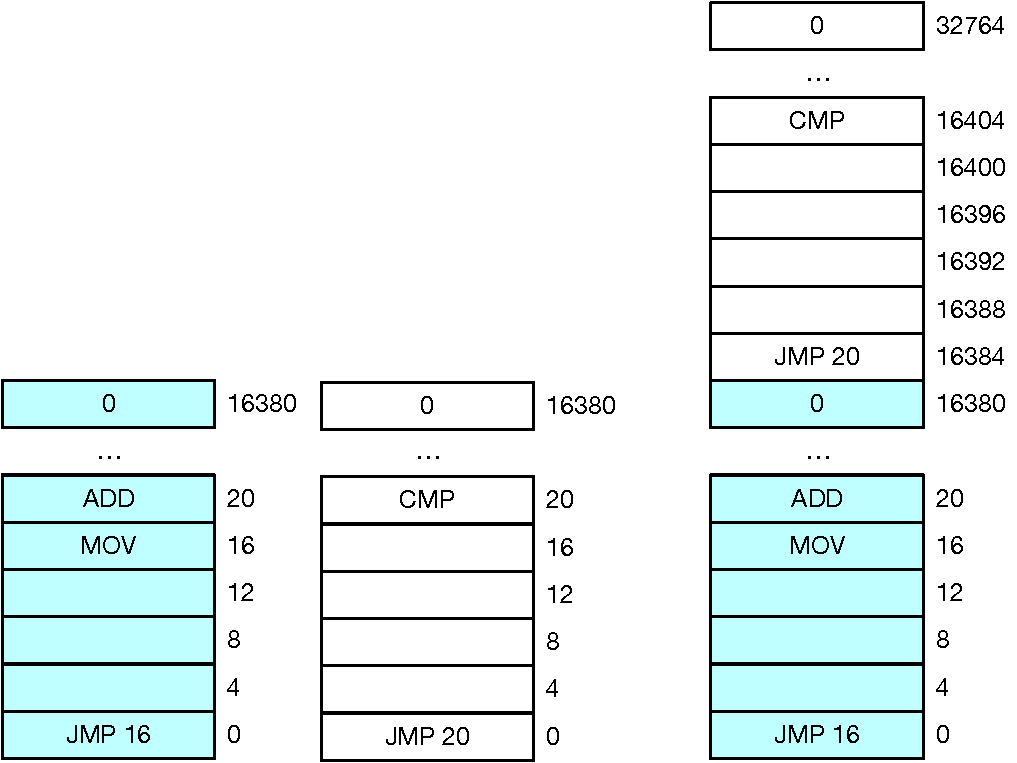
\includegraphics[scale=0.45]{./figures-pdf/multi}
\end{center}

\end{frame}
 %%%%%%%%%%%%%%%%%%%%%%%%%%
\begin{frame}[plain]
\frametitle{Réallocation statique}

\begin{center}
	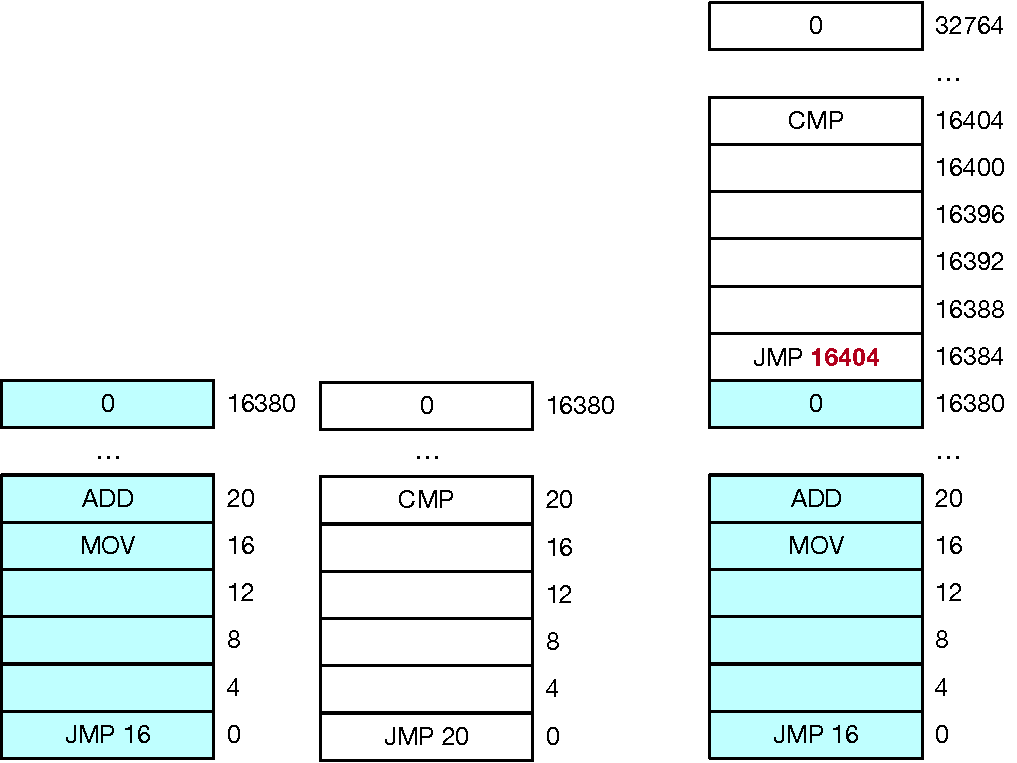
\includegraphics[scale=0.45]{./figures-pdf/statique}
\end{center}

\begin{block}{}
Méthode utilisée pour les systèmes embarqués
\end{block}

\end{frame}

 %%%%%%%%%%%%%%%%%%%%%%%%%%
\begin{frame}[plain]
\frametitle{Espace d'adressage}

\begin{block}{Définition}
Un espace d'adressage est une plage d'adresses valides en mémoire disponibles pour un programme ou un processus, c'est-à-dire que c'est la mémoire à laquelle un programme ou un processus peut accéder.\smallskip

Chaque programme aura son propre espace, ainsi l'adresse 42 d'un programme correspond à un emplacement mémoire différent de l'adresse 42 d'un autre.\smallskip

L'espace d'adressage est une sorte d'abstraction de la mémoire utilisée par un programme. 
\end{block}

\end{frame}

 %%%%%%%%%%%%%%%%%%%%%%%%%%
\begin{frame}[plain]
\frametitle{Réallocation dynamique}

\begin{columns}[t]
  \begin{column}{0.45\textwidth}
	\begin{block}{Définition}
		Ajout de deux registres : registre de base et registre de limite.\smallskip

		A l'exécution le système d'exploitation charge dans ces registres l'adresse physique de début et de fin du programme.\smallskip

		On ajoute à toutes les références mémoires l'adresse de base (et vérifie que l'adresse est inférieure à l'adresse limite).
	\end{block}
	
	\begin{block}{Défaut}
		Nécessite une addition et une comparaison (comparaison rapide mais addition lente -- à cause de la retenue --)
	\end{block}
  \end{column}
  
  \begin{column}{0.45\textwidth}
\begin{center}
	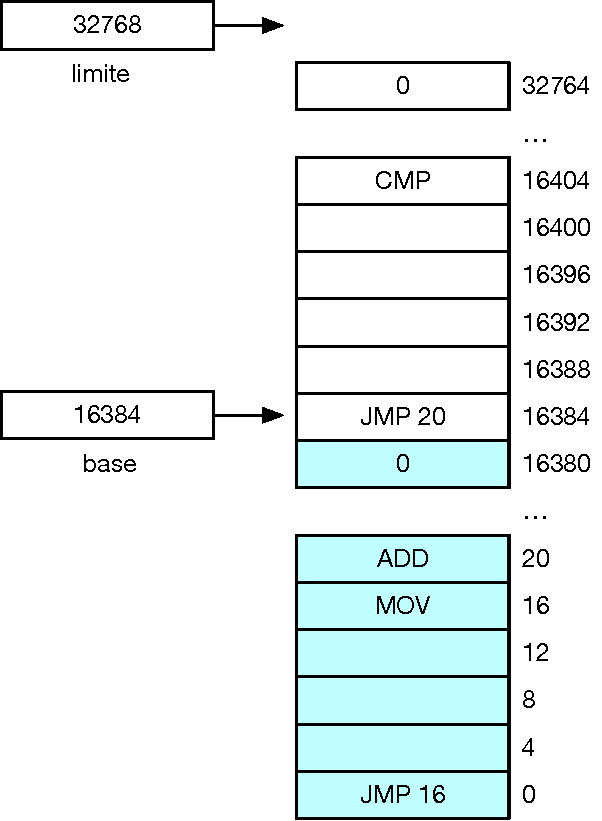
\includegraphics[scale=0.45]{./figures-pdf/base_limite}
\end{center}
  \end{column}
 \end{columns}  

\end{frame}

 %%%%%%%%%%%%%%%%%%%%%%%%%%
\begin{frame}[plain]
\frametitle{Taille de la mémoire}

	\begin{block}{Problème}
		Comment faire si la mémoire physique n'est pas assez grande pour contenir tous les processus ?
	\end{block}
	
	\begin{block}{Solution}
		\begin{itemize}
			\item va-et-vient (swapping)
			\item mémoire virtuelle
		\end{itemize}
	\end{block}

\end{frame}

 %%%%%%%%%%%%%%%%%%%%%%%%%%
\begin{frame}[plain]
\frametitle{Swapping}

\begin{center}
	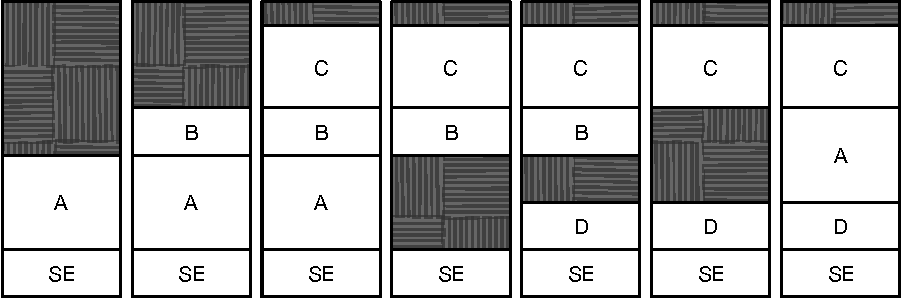
\includegraphics[scale=0.5]{./figures-pdf/swap}
\end{center}

	\begin{block}{}
		\begin{itemize}
			\item réservation d'un espace supplémentaire (tas et pile)
			\item technique de compactage de la mémoire (peu utilisé)
			\item gestion de la mémoire libre : structures (table, listes, etc.) et algorithmes (first fit, next fit, etc.)
		\end{itemize}
	\end{block}

\end{frame}
 %%%%%%%%%%%%%%%%%%%%%%%%%%
\begin{frame}[plain]
\frametitle{Mémoire virtuelle}

	\begin{block}{Principe}
		\begin{itemize}
			\item chaque programme a son espace d'adressage découpé en petites entités, les pages
			\item les pages sont mappées sur la mémoire physique, mais pas forcément toutes les pages pour exécuter le programme
			\item la correspondance entre les adressages virtuels et physiques est fait à la volée par le matériel (Memory Management Unit, MMU)
			\item si une page n'est pas référencée, le système d'exploitation charge l'espace manquant
		\end{itemize}
	\end{block}
\end{frame}

 %%%%%%%%%%%%%%%%%%%%%%%%%%
\begin{frame}[plain]
\frametitle{Pagination}


	\begin{block}{}
		\begin{itemize}
			\item L'espace d'adressage virtuel est divisé en {\bf pages}
			\item Les unités correspondantes dans la mémoire physique sont appelées {\bf cadres de pages} (page frame)
			\item Les pages et les cadres sont de même taille (4ko dans l'exemple)
			\item Les transfert entre la RAM et le disque se font toujours par pages entières
		\end{itemize}
	\end{block}
		
\begin{center}
	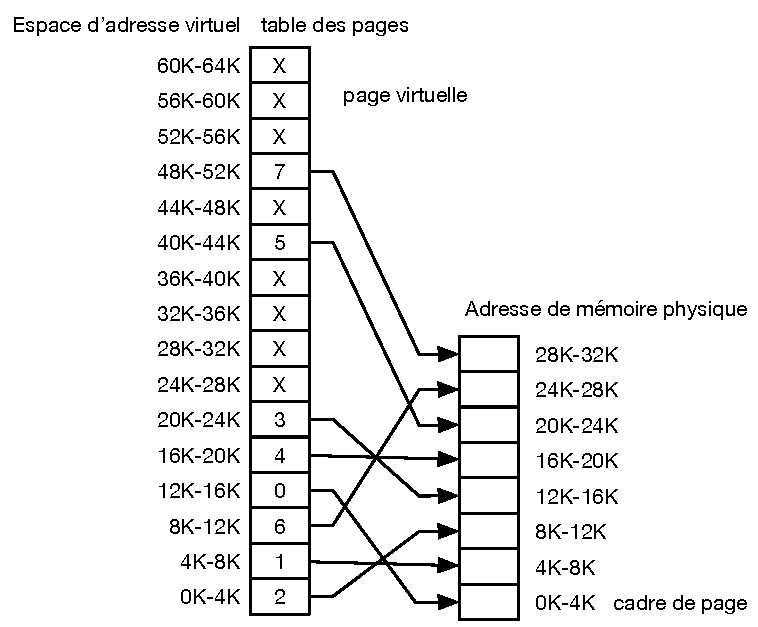
\includegraphics[scale=0.5]{./figures-pdf/pagination}
\end{center}
\end{frame}
 %%%%%%%%%%%%%%%%%%%%%%%%%%
\begin{frame}[plain]
\frametitle{Défaut de page}


	\begin{block}{Algorithme de remplacement de page}
	Une instruction fait un accès à une page qui n'est pas présente
		\begin{enumerate}
			\item sélection d'un cadre de page peu utilisé
			\item écriture sur le disque du cadre sélectionné
			\item transfert de la nouvelle page référencée dans le cadre libéré
			\item modification de la table des pages
			\item poursuite de l'instruction
		\end{enumerate}
	\end{block}

\end{frame}
 %%%%%%%%%%%%%%%%%%%%%%%%%%
\begin{frame}[plain]
\frametitle{TLB (mémoire cache) }

	\begin{block}{Problème}
	La correspondance de pages doit être rapide et est une contrainte de performance
	\end{block}

	\begin{block}{Observation}
	Un programme fait des accès à un petit nombre de pages
	\end{block}

	\begin{block}{Utilisation}
	Mémoire locale à la MMU avec une petite table de correspondance (Translation Lookaside Buffer, TLB).

	Le TLB mémorise les derniers couples (page, cadre) correspondant aux dernières pages auxquelles le processeur a dû accéder, ce qui permet d'améliorer grandement les temps d'accès à la mémoire
	\end{block}

\end{frame}
 %%%%%%%%%%%%%%%%%%%%%%%%%%
\begin{frame}[plain]
\frametitle{Et encore}

	\begin{itemize}
		\item Page des grandes mémoire
		\item Algorithme de remplacement de pages (non récemment utilisée, premier entré-premier sorti , LRU, etc.)
		\item Conception des systèmes de pagination (local/global, taille, séparation instructions et données, etc.)
		\item Pages partagées
		\item Bibliothèques partagées
		\item Segmentation
	\end{itemize}

\end{frame}
 %%%%%%%%%%%%%%%%%%%%%%%%%%

%%%%%%%%%%%%%%%%%%%%%%%%%%
\end{document}